\documentclass[../main.tex]{subfiles}

\begin{document}
	 \section{Einleitung}
	 
	 \subsection{Themenwahl}
	 Die Themenwahl verlief für mich sehr einfach, da mir schon von Anfang an bewusst war, dass ich eine Maturaarbeit im Bereich Wirtschaft und Recht schreiben wollte. 
	 Die Präferenz eine wirtschaftlich-rechtliche Arbeit zu schreiben, mischte ich mit meinen privaten Interessen im Bereich der Drogenpolitik. 
	 Dass die Wahl schlussendlich auf die Droge Cannabis fiel, kann man so erklären, dass der Konsum viele Menschen unserer Gesellschaft betrifft. 
	 Dies konnte ich auch bestätigen, nachdem ich durch die Hilfe von Statistiken die genaueren Zahlen betrachten konnte. 
	 Zur Zeit der Themenfindung waren in Deutschland und teilweise in der Schweiz gesundheitsschädliche synthetische Cannabinoide im Umlauf, was meine Aufmerksamkeit noch weiter auf die Cannabis Legalisierung zog.
	 Anfangs war die Themenwahl sehr breit formuliert und schloss jeden Aspekt einer Legalisierung ein. 
	 Erst beim Erarbeiten der Quellen wurde mir bewusst, wie tiefgründig das Thema ist. 
	 Während der Phase der Erarbeitung der Quellen wurde das Thema immer weiter eingegrenzt, sodass am Ende der Fokus auf dem marktwirtschaftlichen Ansatz der Legalisierung lag. 
	 Das theoretische Konzept einer marktwirtschaftlichen Legalisierung wollte ich dann auf die Schweizer Wirtschaft abbilden.
	 
	 \subsection{Aufbau der Arbeit}
	 Die Einleitung enthält formale Informationen über die Arbeit und bietet dem Leser eine gute Basis für das Verständnis des Inhaltes. 
	 Dem Leser wird ein geschichtlicher Hintergrund über die Prohibition von Cannabis bis hin zur heutigen Zeit vermittelt. 
	 Zudem wird die Schweizer Drogenpolitik in Relation mit anderen Ländern gestellt, um so einen internationalen Vergleich zu machen.
	 Im nächsten Kapitel wird der zurzeit präsente Drogenmarkt, namentlich der illegale Schwarzmarkt, mit ökonomischen Mitteln analysiert. 
	 Dem Leser soll klar werden, nach welchen Prinzipien die Akteure handeln und wie sich die Illegalität auf das Verhalten auswirkt.
	 Die mikroökonomische Analyse des aktuell vorzufindenden Marktes schafft eine Basis für den Vergleich beider Modelle.
	 In der Analyse soll schon klar werden, aufgrund welchen wirtschaftlichen Faktoren eine Prohibition sich positiv aber auch negativ auf den Konsum der Gesellschaft auswirken kann. 
	 Im dritten Kapitel wird ein eigenes Konzept für eine mögliche Legalisierung erarbeitet. 
	 Das Konzept soll dabei möglichst den Werten der Schweizer Rechtsprechung und Politik entsprechen.
	 Der Fokus liegt auf den nötigen Einschränkungen und der nötigen Rechtsprechung.
	 Nebenbei wird eine Analyse zu einem Legalisierten Markt ohne Einschränkungen gemacht.
	 Im Kapitel "Vergleich" werden beide Modelle in Bezug auf die wirtschaftlichen und gesellschaftlichen Auswirkungen miteinander verglichen. 
	 
	 
	 
	 \subsection{Methodik}
	 Die zum grössten Teil vorherrschende Methodik ist die Literaturanalyse, wobei viele Teile auf eigenen Gedankengängen basieren. 
	 So wird für einzelne Zahlen auf bereits vorhandene Studien zurückgegriffen, da spezialisierte Organisationen eine weitaus bessere Datenbasis besitzen und eine höhere Anzahl an Studienteilnehmer befragen können. 
	 Das Ausweichen auf Studien ist mit dem Gesetz der grossen Zahlen zu begründen, dass eigene Studien viel stärker vom tatsächlichen Wert abweichen würden als Studien grosser Organisationen.
	 Die Basis der Arbeit besteht aus Büchern, theoretisch-wissenschaftlichen Arbeiten rund um das Thema Legalisierung und Studien von unabhängigen Organisationen.
	 Die Berechnungen der Arbeit wurden von Hand gemacht und nehmen sich die Datenwerte der Studien zu Hilfe.
	 Das Erarbeiten des eigenen Konzeptes basiert auf eigenen Überlegungen, die sich an der bereits bestehenden Rechtslage anderer psychoaktiven Substanzen orientieren.
	 
	 \subsection{Leitfragen}
	 Die Leitfragen sind wirtschaftlicher und rechtlich-politischer Natur und beschäftigen sich vor allem mit Auswirkungen.
	 Die erste Leitfrage konzentriert sich auf den illegalen Cannabismarkt der Schweiz.
	 Es wird geklärt, wie er aufgebaut ist, wie die Akteure handeln und wie er aus ökonomischer Sicht aussieht.\vspace{0.3cm}
	 \begin{itemize}
	 	\item Wie funktioniert der präsente Cannabismarkt der Schweiz und wie sieht er aus?
	 \end{itemize}\vspace{0.3cm}
	 
	 \noindent
	 Die zweite Leitfrage besteht daraus, wie man eine Legalisierung in der Schweiz durchführen würde und welche Einschränkungen man treffen muss.
	 Dabei werden die Vorstellungen der Schweizer Politik und Gesellschaft miteinbezogen.\vspace{0.3cm}
	 \begin{itemize}
	 	\item Welche Massnahmen muss man treffen, damit eine marktwirtschaftliche Legalisierung den Vorstellungen der Schweizer Politik und Gesellschaft entspricht?
	 \end{itemize}\vspace{0.5cm}
	 
	 \noindent
	 Die dritte Leitfrage fokussiert sich auf die Auswirkungen der Legalisierung und vergleicht sie mit der Prohibition. 
	 Vorteile werden mit den Nachteilen beider Situationen relativiert und bewertet, sodass die Schlussfolgerung die Frage beantworten kann, ob eine Legalisierung sinnvoll ist.\vspace{0.3cm}
	 \begin{itemize}	 
	 	\item Wie unterscheiden sich die Legalisierung und die Prohibition wirtschaftlich und gesellschaftlich?
	 \end{itemize}
	
	 
	 \subsection{Geschichte}
	 Die Schweizer Drogenpolitik begann ab den 1920er Jahren an Bedeutung zu gewinnen. 
	 Der Einstieg stellt dabei die Internationale Opiumkonferenz dar. 
	 Die Internationale Opiumkonferenz führte zum ersten internationalen Abkommen über den Umgang mit Betäubungsmitteln. 
	 Die Opiumkonvention führte jedoch nur zu einem Verbot von Morphin und Kokain. 
	 Weitere Verschärfungen der Drogenpolitik kamen erst 1951, als das Bundesgesetz über die Betäubungsmittel und die psychotropen Stoffe (BetmG) verabschiedet wurde.
	 Seit der Einführung des BetmG ist auch Cannabis als verbotenes Betäubungsmittel klassifiziert.%
	 \footnote{Vgl. \cite{brassel}.}\footnote{Vgl. \cite{admin-01}.}\\
	 	 
	 \noindent
	 Die wichtigste Änderung des BetmG wurde im Jahr 2011 durchgeführt, als die Bevölkerung 2008 dem revidiertem Betäubungsmittelgesetz zustimmte. 
	 Seit der Änderung sind die Viersäulenpolitik und die Behandlungen mit Heroinabgaben feste Bestandteile. 
	 Die Viersäulenpolitik sieht vor, dass neben der Repression auch Massnahmen in Prävention, Schadensminderung und Therapie getroffen werden.
	 So liegt der Schwerpunkt nicht mehr auf der Durchsetzung der Repression, sondern auf dem Wohl der Gesellschaft.
	 Der Konsum wird nicht mehr nur durch das Strafmass gesteuert, sondern auch durch Prävention gemindert. 
	 Bereits erkrankten Menschen werden gesetzlich vorgesehene Massnahmen zur Verfügung gestellt.
	 Der Jugendschutz wurde gestärkt, indem man das Strafmass für den Verkauf an Jugendliche erhöhte.%
	 \footnote{Vgl. \cite{infoset-01}.}\footnote{Vgl. \cite{parlament-01}.}\\
	 
	 \noindent
	 Zur gleichen Zeit wurde über die Volksabstimmung über die Legalisierung von Cannabis abgestimmt.
	 Die Vorlage wurde jedoch von zwei Dritteln der Bevölkerung abgelehnt.
	 Man befürchtete, dass der Drogentourismus stark zunehmen würde, und wollte nicht internationale Abkommen verletzen.
	 Die Befürworter waren nicht überrascht über den Verlust und nahmen die Diskussion gleich wieder auf. 
	 Die neuen Forderungen bestanden aus den Änderungen, dass der Konsum nur noch mit einer Ordnungsbusse bestraft werden kann. 
	 Dies führte zum ersten expliziten Schritt in Richtung einer Legalisierung von Cannabis, sodass die straffreie geringfügige Menge auf 10 Gramm festgesetzt wurde.
	 Der Handel und Besitz hoher Mengen steht immer noch unter Strafe, da man nur Konsumenten und nicht Händler entlasten wollte.%
	 \footnote{Vgl. \cite{infoset-02}.}\footnote{Vgl. \cite{parlament-02}.}
	 
	 
	 \subsection{Heutige Lage}
	 In der jetzigen gesetzlichen Lage ist der Besitz von Cannabis erst ab einer Menge über 10 Gramm strafbar, da es sich dann nicht mehr um eine geringfügige Menge handelt und man annimmt, dass es sich nicht mehr um Eigenkonsum handelt.
	 Der Umgang mit geringfügigen Mengen ist in \texttt{Art. 19b BetmG} geregelt.
	 Der Konsum ist nach \texttt{Art. 19a BetmG} jedoch immer noch strafbar und wird mit einer Ordnungsbusse bestraft \textit{(siehe Abbildung \ref{fig:stgb-art-19})}. 
	 Man kann bei Cannabis inzwischen von einer de facto Legalisierung für Konsumenten reden, da der Konsum gesetzlich gesehen zwar verboten ist, jedoch der Nachweis selten erbracht werden kann. 
	 Alle vom BetmG kontrollierten Substanzen befinden sich seit der Revidierung des Betäubungsmittelgesetzes, das von der Bevölkerung im Jahr 2008 angenommen wurde, in der Betäubungsmittelverzeichnisverordnung (BetmVV-EDI). 
	 So untersteht der Stoff Tetrahydrocannabinol (THC) und teilweise dessen synthetische Analoga der Kontrolle.\vspace{2pt}
	 
	 \begin{figure}[H]
	 \begin{tcolorbox}
	 	\textbf{Art. 19a StGB}\\[7pt]
		1.\quad Wer unbefugt Betäubungsmittel vorsätzlich konsumiert oder wer zum eigenen Konsum eine Widerhandlung im Sinne von Artikel 19 begeht, wird mit Busse bestraft.\\[10pt]
		\ldots
	\end{tcolorbox}
	
	\begin{tcolorbox}
		\textbf{Art. 19b StGB}\\[7pt]
	 	1.\quad Wer nur eine geringfügige Menge eines Betäubungsmittels für den eigenen Konsum vorbereitet oder zur Ermöglichung des gleichzeitigen und gemeinsamen Konsums einer Person von mehr als 18 Jahren unentgeltlich abgibt, ist nicht strafbar.\\[10pt]
2.\quad 10 Gramm eines Betäubungsmittels des Wirkungstyps Cannabis gelten als geringfügige Menge.
	 \end{tcolorbox}
	 \captionsetup{font=small}
	 \caption{Rechtslage von Cannabis in der Schweiz}
	 \label{fig:stgb-art-19}
	 \end{figure}
	 
	 
	 \noindent
	 Cannabis ist mit grossem Abstand die meist konsumierte illegale Droge der Schweiz, obwohl sie dem Betäubungsmittelgesetz untersteht. 
	 Etwa 33.8\% der Schweizer Bevölkerung konsumierte bereits einmal in ihrem Leben Cannabis. 
	 Bei der jungen Bevölkerung sind die Zahlen noch viel höher, sodass bereits die Mehrheit einmal Cannabis konsumiert hat.%
	 \footnote{Vgl. \cite[85]{gmel}.}
	 Das Wachstum der Zahlen ist seit Jahren positiv und es macht auch keinen Anschein, dass diese sich in Zukunft ändern werden.
	 Die hohe Zahl an Konsumenten und die Entwicklung lässt die Frage offen, ob die Prohibition ihrem gewünschten Zweck dient oder ihr Ziel verfehlt.
	 Die Sozioökonomie wird in Kapitel 2.3 genauer erläutert.
	 
	 \noindent
	 Wenn man die Schweiz mit dem Rest der Welt vergleicht, wird man feststellen, dass sich die Schweiz auf der liberalen Seite befindet.
	 Auch in der Gesellschaft herrscht keine generelle Abneigung gegenüber dem Cannabiskonsum und den Konsumenten.	
	 Insgesamt gibt es vier Länder, die Cannabis bereits legalisiert haben.
	 Diese Länder sind Uruguay, Kanada, Südafrika und Georgien, wovon auf 3 dieser Länder noch Bezug genommen wird.
	 Die Schweiz gehört zu der Gruppe bestehend aus 49 weiteren Staaten, die Cannabis zwar entkriminalisiert haben und teilweise dulden, jedoch rechtlich nicht legalisiert haben. \textit{(Siehe Abbildung \ref{fig:worldwide})}\\
	 
	 \noindent
	 \begin{figure}[H]
	 	\centering
	 	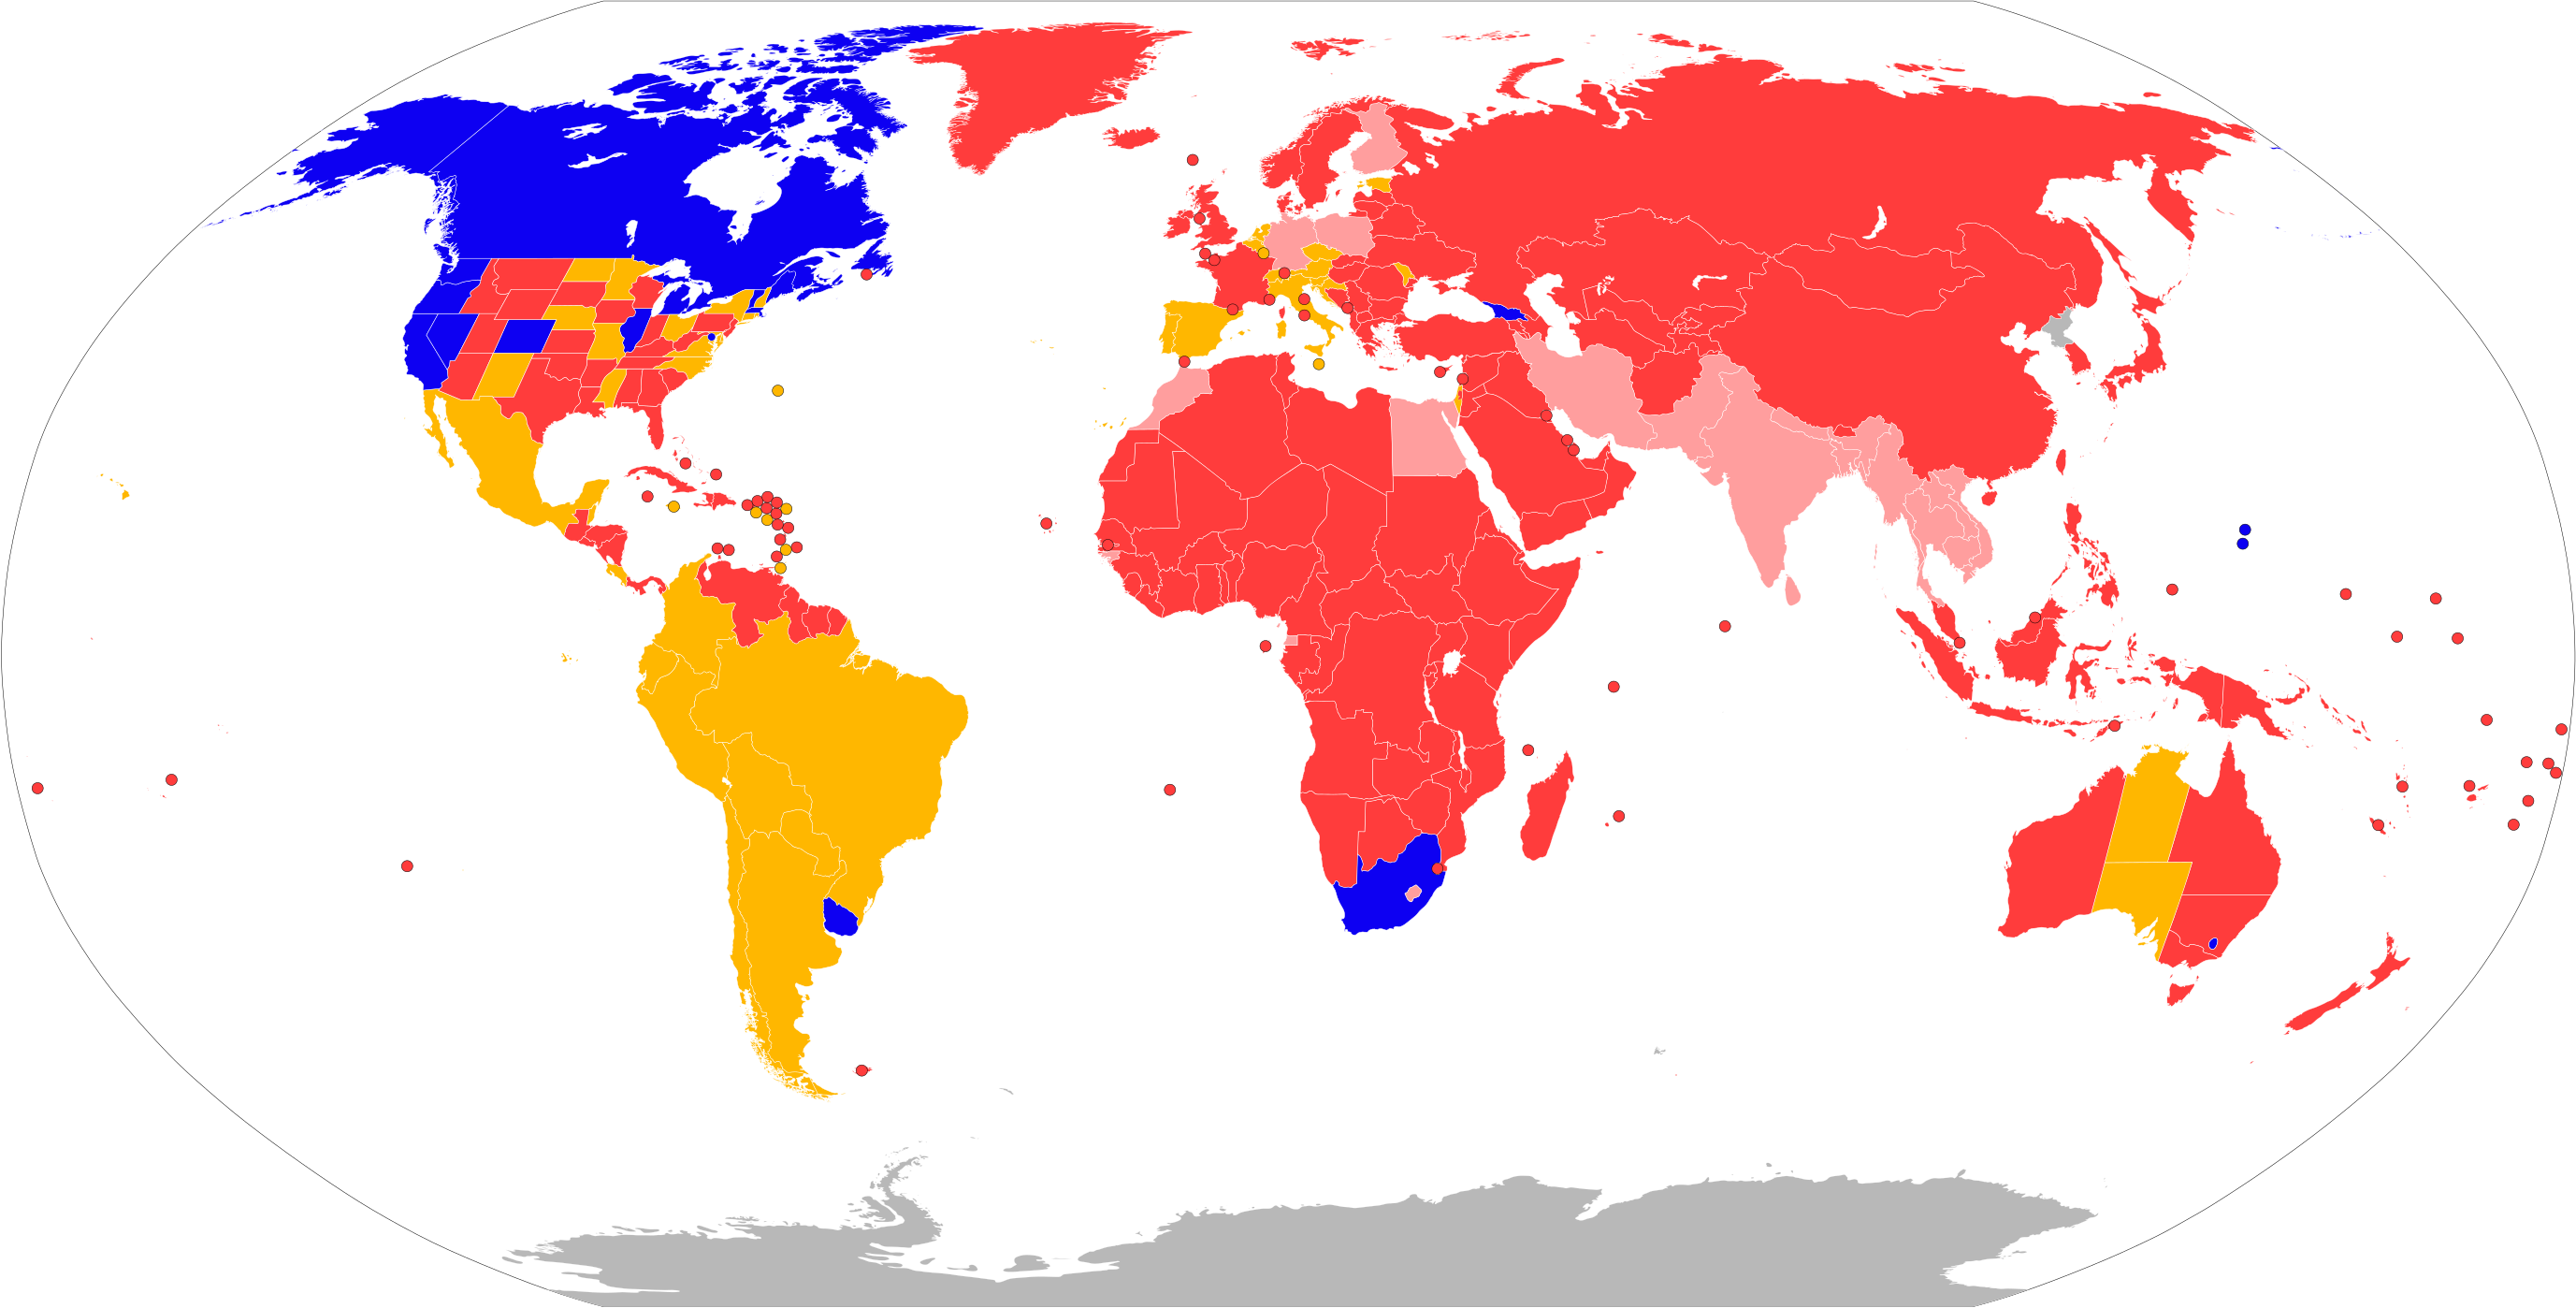
\includegraphics[width=0.9\linewidth]{CannabisWeltweit}\\[7pt]
	 	
		\fcolorbox{black}[HTML]{ff3c3c}{\rule{0pt}{6pt}\rule{6pt}{0pt}}\hspace{0.8em} Illegal \hspace{2.5em}
	 	\fcolorbox{black}[HTML]{ff9e9e}{\rule{0pt}{6pt}\rule{6pt}{0pt}}\hspace{0.8em} Keine zwingende Strafverfolgung \hspace{2.5em}
	 	\fcolorbox{black}[HTML]{ffb700}{\rule{0pt}{6pt}\rule{6pt}{0pt}}\hspace{0.8em} Entkriminalisiert\\[5pt]
	 	\fcolorbox{black}[HTML]{0d00f2}{\rule{0pt}{6pt}\rule{6pt}{0pt}}\hspace{0.8em} Legal \hspace{2.5em}
	 	\fcolorbox{black}[HTML]{b6b6b6}{\rule{0pt}{6pt}\rule{6pt}{0pt}}\hspace{0.8em} Keine Information	 	
	 	
	 	\captionsetup{font=small}
	 	\caption[Rechtslage von Cannabis weltweit]{Rechtslage von Cannabis weltweit\protect\footnotemark}
	 	\label{fig:worldwide}
	 \end{figure}
	 
	 \noindent
	 
	 
	 \footnotetext{\cite{wikipedia-01}.}
	 
\end{document}